\documentclass[class=jsarticle, crop=false, dvipdfmx, fleqn]{standalone}
\input{/Users/User/Documents/TeX/preamble/mypreamble}
\begin{document}
\section*{練習問題4-5}

温度変化のモデルを,
\begin{align}
& T(t) = T_0 + a\sin(\omega t + \theta) + \varepsilon (t) \\
& \varepsilon (t) \sim N(0, \sigma^2)
\end{align}
として,パラメータ$T_0,\ a,\ \omega,\ \theta,\ {\sigma^2}$を最尤推定する。
ここで,誤差項$\varepsilon (t)$が正規分布に従うから,
最尤法による解と最小二乗法による解は一致する。
よって最小二乗法によってこれらのパラメータを求めることとする。

最小二乗法にはPythonのscipy.optimize.leastsqを用いた。
また,それぞれのパラメータの初期値は,
元データを概算で読み取り,それぞれ以下のようにした。
\begin{align*}
& T_0 = 13, \qquad a = 3.0 \\
& \omega = 2\pi/6000, \qquad \theta = 0.0
\end{align*}

最尤推定の結果は以下のようになった。

\begin{table}[H]
\centering
\caption{【練習問題4-5】 最小二乗法によるパラメータ推定の結果}
\begin{tabular}{lcr}
$T_0\unitis{\celsius}$ & : & 12.67 \\
$a\unitis{\celsius}$ & : & 2.916 \\
$\omega\unitis{/s}$ & : & 0.001059 \\
$\theta$ & : & -0.1846 \\
%$\mu$ & : & -5.29456656295224e-10 \\
${\sigma}^2$ & : & 0.3171
\end{tabular}
\label{tab:q4-5_result}
\end{table}

\begin{figure}[H]
\centering
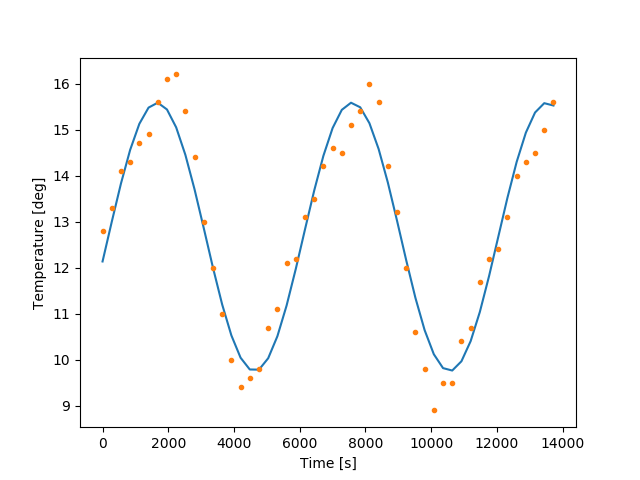
\includegraphics[clip, width=12cm]{../figures/q_4_5_2}
\caption{【練習問題4-5】 最尤推定によって求めたモデルのプロット}
\label{fig:q4-5-2_graph}
\end{figure}


\end{document}